\section{Server Application}

This section discusses the~design aspects of the~server application of the~designed game.
It discusses the~design of an~API server.
Then the~server architecture is described and designed according to previous chapters.
There is a~discussion on different framework options and how the~framework works with entities and DTOs.
Then there is a~discussion about controllers, repositories, and services.
And finally, a~note about tokens.

\subsection{Web API}

Application Programming Interface (API) is an~interface with a~set of functions that can be used to get data from an~application~\cite{a2022_aspnet}.
API accessed over the~web using the~HTTP protocol is called Web API.
They can be developed with different technologies like ASP.NET, Java, Python, etc.
A web API can be used from a~mobile, desktop, web, or any other application or game using the~HTTP protocol.
Web API can also use other web APIs.

One of the~representatives of web API is ASP.NET Web API~\cite{a2022_aspnet}.
It is a~web framework that is often used to create websites and APIs using languages such as C\#.
The~framework supports an~automatic serialization of data classes into the~JSON format.
It supports built-in support for authentication and authorization with built-in support for standards such as JSON Web Tokens (JWT).
It also provides multiple annotations for use inline with the~code, like routing annotations that let developers mark methods that should provide routing.

The~ASP.NET Web API framework will be used in the~server part of the~designed game for its simplicity and industry-level power.

\subsection{Architecture}

As mentioned in chapter~\ref{design:architecture:clean-archiecture}, the~server application will follow the~principles mentioned in the~Clean Architecture.
It is divided into multiple layers: data layer, repositories contracts layers and repositories layer, services contracts layer and services layer, and controllers layers.

\begin{figure}
    \centering
    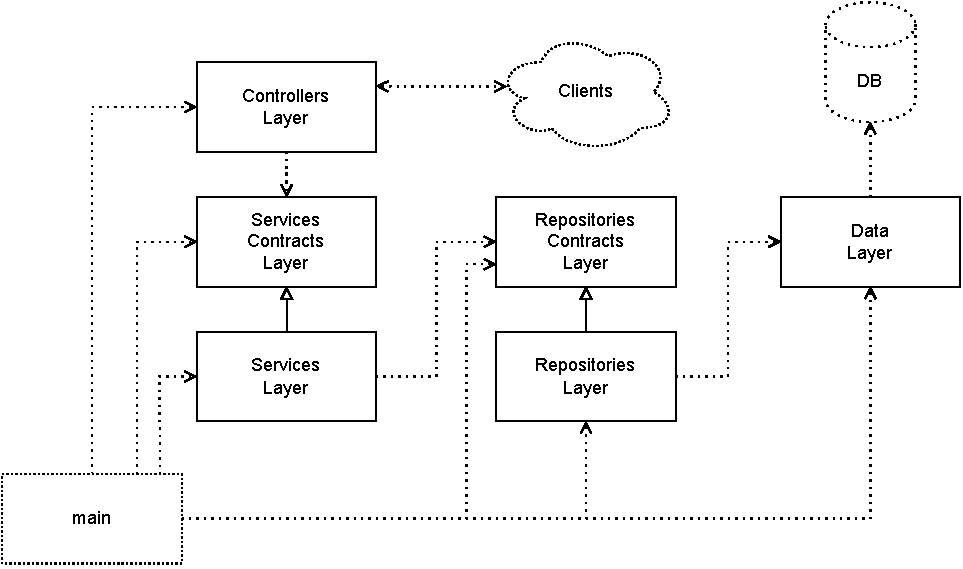
\includegraphics[width=1\linewidth]{assets/design/serverarchitecture.pdf}
    \caption{Server Architecture}
    \label{fig:design:serverarchitecture}
\end{figure}

The~data layer declares entities and their mapping.
Entities should use Object-Relational Mapping (ORM) to map themselves to the~database model.
Using the~ASP.NET and its Entity Framework, setting up entities and mapping is very straightforward.
The~Entity Framework recognizes the~primary identification and translates all attributes and their types to corresponding database types.

The~repositories contracts layer contains repositories' interfaces.
They are used to provide basic methods for communication with the~database.
These interfaces do not use any code from other layers.

The~repositories layer contains the~repositories contracts layer's implementation of the~repositories.
These implementations return Data Transfer Objects (DTOs) after processing entities fetched from the~database.

The~services contracts layer contains services' interfaces.
They are used as a~layer between controllers and repositories.
These interfaces do not use any code from other layers.

The~services layer contains the~services contracts layer's implementation of the~services.
These implementations use repositories contracts passed in their constructors using the~dependency injection.

The~controllers layer provides Web API controllers that processes work using services.

As you can see from the~description and the~figure~\ref{fig:design:serverarchitecture}, the~server architecture follows the~SOLID principles, mainly the~dependency inversion principle.

\subsection{Entities and DTOs}

The~Entity Framework is an~open-source data access framework.
It does Object-Relational Mapping (ORM), so developers can use the~database as with objects~\cite{a2021_overview}.
The~framework also reduces the~direct data access needed and exposes a~high-level interface.

The~database model consists of entities and the~database context object~\cite{a2022_creating}.
The~context object represents the~database relations.
Entities are ordinary data objects.
Each entity is registered as \mintinline{text}|DbSet<Entity>| attribute with a~getter and a~setter.
The~context can set up entity mappers using the~Fluent API, as can be seen in the~code~\ref{fig:database-context}.
The~Fluent API is a~method of modifying the~model without changing the~entity class.
It also has higher precedence than annotations that can be used directly on entity class and its attributes.

\begin{listing}
    \caption{Sample Database Context}
    \label{fig:database-context}
    \begin{minted}{csharp}
internal class MyContext : DbContext
{
    public DbSet<User> Users { get; set; }

    protected override void OnModelCreating(
        ModelBuilder modelBuilder
    )
    {
        modelBuilder.Entity<User>()
            .HasIndex(u => u.Username)
            .IsUnique();
    }
}
    \end{minted}
\end{listing}

Querying data from the~database with the~Entity Framework can be done using the~Language-Integrated Query (LINQ).
LINQ queries are strongly typed, and it is as simple as calling methods in the~database context.
Because methods returns live queries, it is recommended to await the~query as a~collection to finish the~fetching.

Entities are mapped from the~database.
Entities are transformed into Data Transfer Objects (DTO) to handle incoming and outcoming data.
DTOs always contain only data needed for further processing to prevent sending unnecessary data.

The~typical scenario flow might be that a~controller is triggered, it calls a~service, which calls a~repository.
The~repository does a~fetch to the~database, and data are stored in a~collection and later transformed into DTOs.
DTOs are returned from the~repository and processed by the~service.
After processing, the~data are returned to the~controller, creating a~response containing those data.

\subsection{Controllers}

Controllers provide Web APIs that process requests using services from the~services layer delivered to the~services contracts layers using the~dependency injection tool.
Controllers should be designed to cover all use cases of the~developed game.

There should be a~controller for the~authentication of users.
That means signing in and signing up for the~game.
These API endpoints should be allowed to be run anonymously.
If the~sign-in or sign-up processes finish successfully, a~JWT token should be generated and returned as a~response with user data.

The~user controller should contain endpoints to get a~user by id, get a~user by username and get a~user by the~token.
These endpoints should be locked and available only to authenticated users.
Each endpoint should return a~user object.

The~story controller should be able to get all stories and a~story by its id.
Based on the~endpoint, different data should be returned.
The~get-all-stories endpoint should return a~list of stories.
The~get-story-by-id endpoint should return a~story with all of its missions.
These endpoints should be locked and available only to authenticated users.

Similarly, the~mission controller should also be able to get all missions and a~specific mission.
Both endpoints return game, learning, or storytelling mission.
Additionally, it should also have an~endpoint to update the~game result.
These endpoints should be locked and available only to authenticated users.

And finally, the~stats endpoint should return stats for all stories and their mission for the~authenticated user.
This endpoint should be locked and available only to authenticated users.

\subsection{Services}

Services handle requests from controllers.
They are the~middleware between controllers and repositories and handle additional logic.
There should be three types of services: a~user service, a~story service, and a~token service.

The~user service should be able to get a~user by their id or username.
It should also process login and register processes.
This service should also know how to hash and verify users' passwords.

The~story service should contain methods to get story and stories, mission and missions, and save game progress.
Their URL attribute differentiates the~mission and the~story.
If requesting all missions, a~story URL must be provided.
All stories do not need additional data.

The~token service needs to contain the~generation of a~token and its verification.
The~token is generated based on the~user data object.
And the~verification is done by passing the~token.

\subsection{Repositories}

There should be at least two repositories for stories and users.
The~user repository should contain creating a~new user and getting a~user by their id or username.
The~story repository should contain all methods to fetch and modify stories and missions.
Getting all stories, getting a~specific story by its story URL, getting all missions by their story URL, and getting a~particular mission by its URL.
It should also provide getting stories' stats for a~user.
And the~save game progress.

\subsection{Tokens}
\label{design:server:tokens}

User authentication is done either by sessions or tokens.
These two methods do a~similar job, but servers manage sessions, and clients manage tokens.
Both methods can deal with authentication and authorization.
Authentication verifies that a~user is who they say they are.
That can be done by providing a~password or a~fingerprint.
Authorization verifies that a~user has permission to do things.
It is a~way to allow a~user to access some locked resource.~\cite{lin_2018_tuck}

Tokens deals with the~authorization of APIs.
Typically JSON Web Tokens (JWT) are used to secure APIs.
JWT is an~open security standard that allows the~secure transmission of data~\cite{lin_2018_tuck}.
JWT is added to an~authorization header \mintinline{text}|Authorization: Bearer <jwt-token>| on the~client's request, and the~server then reads it and verifies it.
A schema of JWT lifetime can be seen in the~figure~\ref{fig:design:jwt}.

\begin{figure}
    \centering
    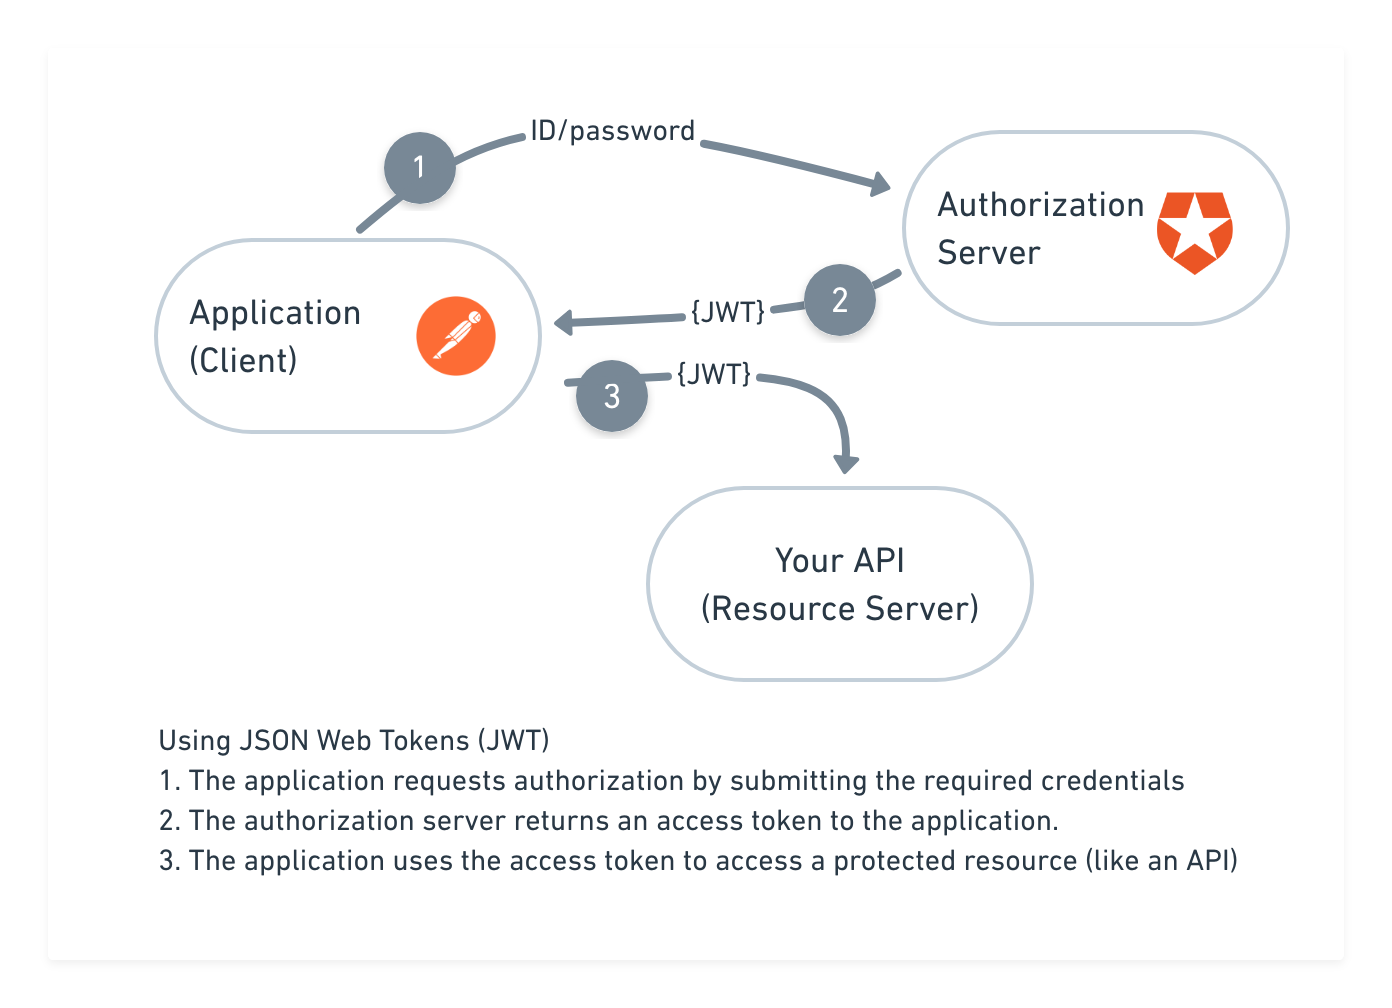
\includegraphics[width=1\linewidth]{assets/design/jwt.png}
    \caption{JSON Web Tokens~\cite{lin_2018_tuck}}
    \label{fig:design:jwt}
\end{figure}

Users will be forced to sign in using their username and password combinations to authenticate.
The~game verifies that the~user is who they say they are.
Then, the~game saves the~JWT token from the~response, and from now on, it uses the~token to authorize the~request to the~Web API.
